\begin{usecase}{Suggest Conflict Resolutions}
	\ucbasicinfo{High}{Regular}
	\ucshortdescription{This UC provides users with conflict detection and resolution options for calendar events.}
	\uctrigger{The UC is triggered when a new event is added that overlaps with existing events}
	\ucactors{User}{iOS App}{Backend Service}
	\ucpreconditions{
		\begin{itemize}
			\item The user has calendar access authorized
			\item The user has notifications enabled
			\item The calendar contains at least one event
		\end{itemize}
	}
	\ucrelationships{N/A}{Manage Scheduling Conflicts}{N/A}
	\ucinputsoutputs{
		\begin{itemize}
			\item \textbf{Event details} (Source: Calendar)
			\item \textbf{User resolution choice} (Source: User Interface)
		\end{itemize}
	}{
		\begin{itemize}
			\item \textbf{Updated calendar events} (Destination: Calendar)
			\item \textbf{Conflict notifications} (Destination: User Device)
		\end{itemize}
	}
	\ucmainflow{
		\begin{enumerate}
			\item The backend service sends event details to the iOS app via push notification
			      \ucinfo{When a new event is added, the backend sends both a visible notification and background event data.}
			\item The iOS app checks for conflicts
			      \ucinfo{The app processes the event data in the background to detect overlaps with existing events.}
			\item The iOS app notifies the user about conflicts
			      \ucinfo{If conflicts are found, a notification is shown to the user.}
			\item The app presents resolution options
			      \ucinfo{When the user opens the conflict notification, they are presented with three options:
				      \begin{itemize}
					      \item Keep all events (with conflict warning)
					      \item Reschedule the new event to a different time
					      \item Cancel the new event
				      \end{itemize}}
			\item The user selects a resolution option
			      \ucinfo{The system provides a visual timeline to help users understand the conflict and make an informed decision.}
			\item The system applies the chosen resolution
			      \ucinfo{The calendar is updated according to the user's choice:
				      \begin{itemize}
					      \item If keeping both, events are marked as conflicting
					      \item If rescheduling, the event is moved to the new time
					      \item If canceling, the new event is removed
				      \end{itemize}}
		\end{enumerate}
	}
	\ucalternateflows{
		\begin{enumerate}
			\item {No conflicts detected}
			      \ucinfo{If no overlapping events are found, the event is added normally without user intervention.}
			\item {User ignores conflict notification}
			      \ucinfo{Conflicts remain in the app's conflict manager and can be resolved later from the conflicts view.}
		\end{enumerate}
	}
	\ucexceptions{
		\begin{itemize}
			\item If calendar access is not authorized, conflict detection cannot proceed
			\item If notifications are disabled, the user won't be notified of conflicts immediately
			\item If event modification fails, the system retains the conflict state for later resolution
		\end{itemize}
	}
	\ucconclusion{The UC ends when either the conflict is resolved according to user choice, or the conflict is retained for later resolution.}
	\ucpostconditions{
		\begin{itemize}
			\item The calendar reflects the user's chosen resolution
			\item The conflict is marked as resolved in the conflict manager if user acted on it
			\item The conflicts view is updated accordingly
		\end{itemize}
	}
	\ucspecialrequirements{
		\begin{itemize}
			\item The system must provide real-time visual feedback of conflicts using the timeline view
			\item The conflict resolution interface must be intuitive and user-friendly
			\item The system must handle background event processing with best 
		\end{itemize}
	}
\end{usecase}

\begin{figure}[!h]
	\centering
	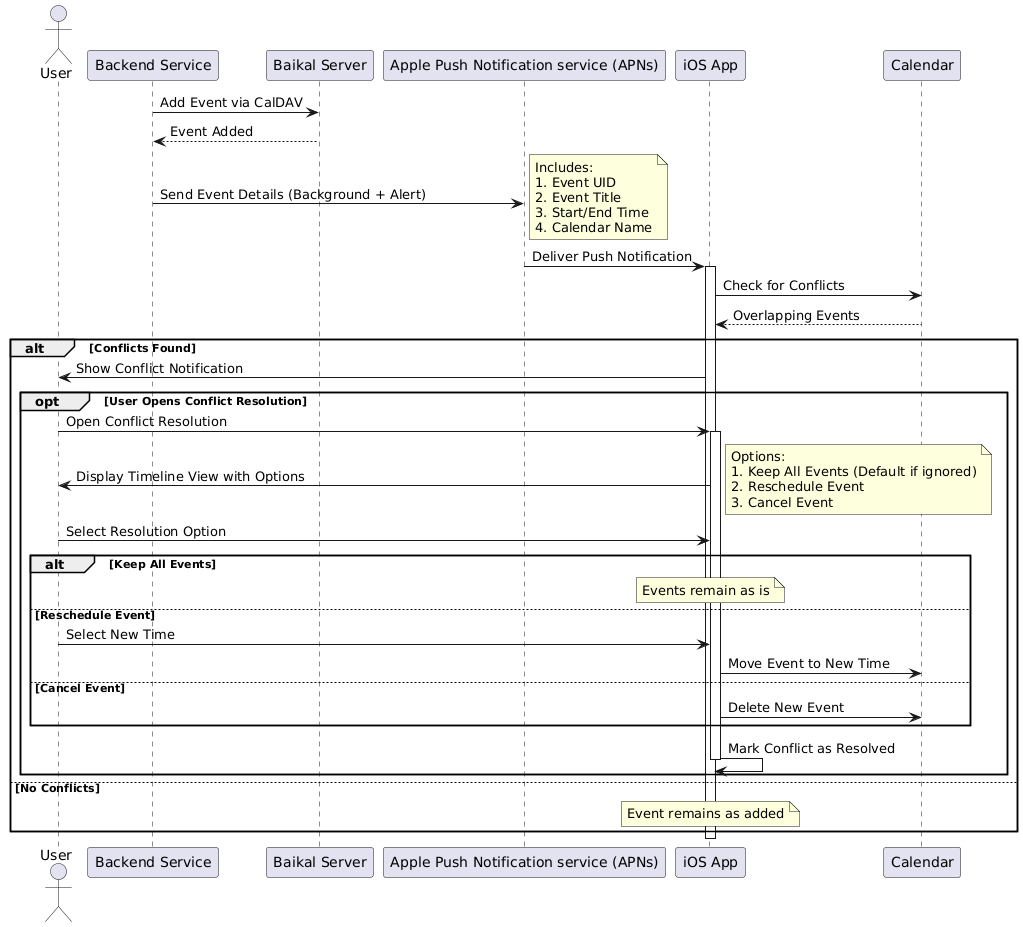
\includegraphics[width=\textwidth]{images/docs/diagrams/sequence-diagrams/all-sequence-diagrams/Suggest Conflict Resolutions.png}
	\caption{Suggest Conflict Resolutions Sequence Diagram}
	\label{fig:seq/suggest-conflict-resolutions}
\end{figure}

The sequence diagram in Figure~\ref{fig:seq/suggest-conflict-resolutions} illustrates the conflict detection and resolution workflow in Jadwal. The process begins when a new event is added to the calendar, particularly through WhatsApp extraction. The backend service sends both a visible notification and background event data through Apple Push Notification service (APNs).

The iOS app implements a sophisticated conflict resolution system that:
\begin{enumerate}
	\item Processes background notifications to detect conflicts
	\item Maintains a conflict manager to track and handle conflicts
	\item Provides a visual timeline interface for understanding conflicts
	\item Offers three resolution options:
	      \begin{itemize}
		      \item Keep all events with an explicit conflict warning
		      \item Reschedule the new event to a different time
		      \item Cancel the new event
	      \end{itemize}
\end{enumerate}

The implementation focuses on user experience by:
\begin{itemize}
	\item Providing immediate notification of conflicts
	\item Offering a visual timeline to understand event overlaps
	\item Allowing flexible resolution timing (immediate or later)
	\item Maintaining a dedicated conflicts view for managing all unresolved conflicts
\end{itemize}

This approach ensures users have complete control over their calendar while being promptly informed of scheduling conflicts. The system maintains conflicts until explicitly resolved, allowing users to make decisions at their convenience while ensuring no scheduling issues go unnoticed.